
\documentclass[]{spie}  %>>> use for US letter paper
%%\documentclass[a4paper]{spie}  %>>> use this instead for A4 paper
%%\documentclass[nocompress]{spie}  %>>> to avoid compression of citations
%% \addtolength{\voffset}{9mm}   %>>> moves text field down
%% \renewcommand{\baselinestretch}{1.65}   %>>> 1.65 for double spacing, 1.25 for 1.5 spacing 
%  The following command loads a graphics package to include images 
%  in the document. It may be necessary to specify a DVI driver option,
%  e.g., [dvips], but that may be inappropriate for some LaTeX 
%  installations. 
\usepackage[]{graphicx}
\usepackage{subfigure}
\usepackage{amsmath}
\usepackage{hyperref}


\graphicspath{{./images/}}

\title{Federating Heterogeneous Datasets to Enhance Data Sharing and Experiment Reproducibility} 

\author{Juan C. Prieto.\supit{a}, Beatriz Paniagua.\supit{a}, Marilia S. Yatabe.\supit{b}, Antonio C.O Ruellas.\supit{b}, 
Liana Fattori.\supit{b}, Luciana Muniz.\supit{b}, Martin Styner.\supit{a}, and Lucia Cevidanes.\supit{c}
\skiplinehalf
\supit{a}NIRAL, UNC, Chapel Hill, North Carolina, United States; 
\supit{b}DCBIA, UMICH, Ann Arbor, Michigan, United States;
}

%>>>> Further information about the authors, other than their 
%  institution and addresses, should be included as a footnote, 
%  which is facilitated by the \authorinfo{} command.

\authorinfo{Further author information: (Send correspondence to J.C.P)\\J.C.P.: E-mail: jprieto@med.unc.edu}
%%>>>> when using amstex, you need to use @@ instead of @
 

%%%%%%%%%%%%%%%%%%%%%%%%%%%%%%%%%%%%%%%%%%%%%%%%%%%%%%%%%%%%% 
%>>>> uncomment following for page numbers
% \pagestyle{plain}    
%>>>> uncomment following to start page numbering at 301 
%\setcounter{page}{301} 
 
  \begin{document} 
  \maketitle 

%%%%%%%%%%%%%%%%%%%%%%%%%%%%%%%%%%%%%%%%%%%%%%%%%%%%%%%%%%%%% 
\begin{abstract}

Recent studies have demonstrated the difficulties to replicate scientific findings and/or experiments published in past\cite{open2015estimating}. 
The effects seen in the replicated experiments were smaller than previously reported. Some of the explanations 
for these findings include the complexity of the experimental design and the pressure on researches to report positive findings. 
The International Committee of Medical Journal Editors (ICMJE) suggests that every study considered for publication must 
submit a plan to share the de-identified patient data no later than 6 months after publication. 
There is a growing demand to enhance the management of clinical data, facilitate data sharing across institutions and also to keep track 
of the data from previous experiments. The ultimate goal is to assure the reproducibility of experiments in the future.
This paper describes Shiny-tooth, a web based application created to improve clinical data acquisition during the clinical trial; 
data federation of such data as well as morphological data derived from medical images; 
Currently, this application is being used to store clinical data from an osteoarthritis (OA) study. 
This work is submitted to the SPIE Biomedical Applications in Molecular, Structural, and Functional Imaging conference.

\end{abstract}

%>>>> Include a list of keywords after the abstract 

\keywords{Data federation, reproducibility, clinical data, sharing, de-identified, web visualization}

%%%%%%%%%%%%%%%%%%%%%%%%%%%%%%%%%%%%%%%%%%%%%%%%%%%%%%%%%%%%%
\section{INTRODUCTION}
\label{sec:intro}

The primary motivation of this work is to improve the state of clinical research data organization in order to facilitate data sharing across institutions and collaborators and ultimately to facilitate the reproducibility of clinical trials.
A number of issues have been identified when working and managing clinical data recorded during clinical trials funded by the National Institute of Health 
(NIH) or private institutions. Frequently, clinical data is recorded and stored in spreadsheets by the clinicians. Very often, before the data analysis begins, 
a significant amount of time is needed to parse, format and detect outliers in the data in order to produce a dataset suited for analysis.
After the analysis is completed and the results have been published, in the majority of cases, 
the clinical data is not public and/or shared beyond the data holder and collaborators. 
This situation has drawn the attention of the scientific community due to the fact that many scientific findings cannot be easily replicated by other groups. 
As time progresses, the reproducibility of a study decreases for a number of reasons: losing track of the location of the data, the scientist is mutated to another institution and/or the the data needs to be reprocessed. As shown by The Open Science Foundation, in an effort to replicate 100 experiments reported in psychological science during 2008\cite{open2015estimating}, about one-third to one-half of the original findings were also observed in the replication studies. 
Similar patterns can be observed in other areas such as cancer research and engineering. 
After the experiments were replicated, the effects seen were smaller than previously reported. 
Some of the explanations for these findings include the complexity of the experimental design and the pressure on researches to report positive findings. 
Recent guidelines proposed by The International Committee of Medical Journal Editors (ICMJE) suggests that a study considered for publication should 
contain a plan to share the de-identified patient data (IPD) and also supplementary material no later than 6 months 
after publication\cite{doi:10.1001/jama.2015.18164}. The main goal is to improve the transparency and robustness of the publications. 
Today, there is a growing demand to enhance the Clinical Data Management (CDM) \cite{krishnankutty_data_2012} in the scientific community. 
CDM describes the processes to maintain high-quality and reliable data from clinical trials.  
Some of the procedures in CDM include data annotation, database design, data validation etc. 
Recent advancements in web technologies could provide the necessary means to generate publicly available tools and/or services to 
facilitate data sharing across institutions, keep track of data from previous experiments and more importantly to 
assure the reproducibility of experiments in the future.
This paper describes Shiny-tooth, a web based application created to improve clinical data acquisition during the clinical trial; 
data federation of such data as well as morphological data derived from medical images; and interactive visualization 
of the clinical data and morphological data stored in a NoSQL database (couchdb). This NoSQL database stores information using Javascript Object Notation 
(JSON) format and offers a document-based query and indexing mechanism. Additionally, couchdb allows attaching binary data to the documents, i.e., medical images, tessellations, etc.; it is implemented following Representational State Transfer (REST) architecture to insert, modify, retrieve and delete records; 
and offers a synchronization feature between two couchdb instances.
Additional frameworks have been used to develop the application, the following section describes its architecture. Currently, this application is being used to store clinical data from an osteoarthritis (OA) study. OA is the most prevalent arthritis worldwide, is associated with significant pain and disability and affects 13.9\% of adults at any given time. OA is very complex and the pathogenesis of TMJ OA remains unclear to this day. OA affects the temporomandibular joint (TMJ), among other joints. TMJ OA represents 42.6\% of the diagnosed disorders of the TMJ, and results in \$4 billion annual health care costs in the US\cite{Cevidanes2010110}\cite{Paniagua2011345}. 

\section{METHODS} 
\label{sec:METHODS}

Shiny-tooth is focused on the re-usability of components and creating a robust and scalable application. 
The backend of the application uses: Node.js \footnote{\url{https://nodejs.org/en/}} as the Javascript engine to run the application; Hapi.js \footnote{\url{http://hapijs.com/}} built on top of node.js, provides REST services and orchestrates communication between components; Couchdb \footnote{\url{http://couchdb.apache.org/}}, for storage and data federation; and Json Web Tokens (JWT) \footnote{\url{https://jwt.io/}} for stateless user authentication in the system.
This framework facilitates the development and integration of plugins in order to generate new services 
in a distributed environment. Hapi.js orchestrates the requests sent by the client 
to the different services deployed in the server including authentication, fetching static and dynamic content, and storage and retrieval of documents from couchdb. Additional plugins such as clusterpost-lib \footnote{\url{https://www.npmjs.com/package/clusterpost-lib}} can be easily integrated in the future allowing shiny-tooth to submit tasks to remote computing grids using the data stored in couchdb.
The front end of the application is based on Angular.js\footnote{\url{https://angularjs.org/}}, this framework facilitates the development of reusable HTML components.
The clinical data visualization is done using D3.js and 3D visualization of morphological data is accomplished with Threejs.
The application is hosted using Amazon web services or the Elastic Computing Cloud (EC2). Shiny-tooth has been applied to store clinical OA data. 

\section{MATERIALS}

The current study consists of 218 TMJ joints, (153 TMJ OA, 65 Controls) obtained from CBCT 
images. Label maps of the TMJs were generated and point distribution models (PDM) with 1002 correspondent 
points were constructed using SPHARM-PDM\cite{Styner2006}. Previously acquired data has been added to the repository and incoming data is being recorded directly in the system.
The following section shows the result of this work. 

\section{RESULTS} 

Figure \ref{fig:serverArchitectureOut} shows the architecture of the application. In green, the plugins that are currently used which include: Hapi-jwt-couch to validate users with JWT and storage of encrypted user passwords in couchdb; shiny-tooth-static serves the static content (HTML) pages to the client; shiny-tooth-model handles storage and retrieval requests of clinical data and morphological data in couchdb. 
In yellow, clusterpost-lib is a plugin that can be deployed in the future in order to submit computational tasks to remote computing grids. 

\begin{figure}
	\centering 
	\includegraphics[width=8cm]{serverArchitectureOut.eps}
	\caption[Server architecture]{Server architecture based on plugins for a distributed application. In green, the plugins that are currently used. In yellow, the plugins that can be integrated in the future.}
	\label{fig:serverArchitectureOut}
\end{figure} 

Figure \ref{fig:gnerateClinicalData} shows the procedure to create data for the current clinical study. 
\ref{fig:gnerateClinicalData}.a shows a collection of Biological Markers. A Collection in this system is defined as a group of clinical data. Nevertheless, 
each JSON document is indexed separately and may be retrieved using the document's content. A collection may be utilized to facilitate the retrieval of meaningful datasets in a study. \ref{fig:gnerateClinicalData}.b shows an extract from a form used to acquire patient information. 
\ref{fig:gnerateClinicalData}.c displays the clinical data in a table format. Another feature of the system is the possibility to import previously acquired data in spreadsheets. However, the content of the spreadsheet must be converted to a comma separated value (CSV) format with the first row being the table header. The header or column names will be used to index the data in the future. If the data is imported from a spreadsheet, it is necessary to specify the column that contains the anonymization id. This id will be used to index the JSON document and perform joints between clinical and morphological data.

\begin{figure}
	\centering 
	\subfigure[]{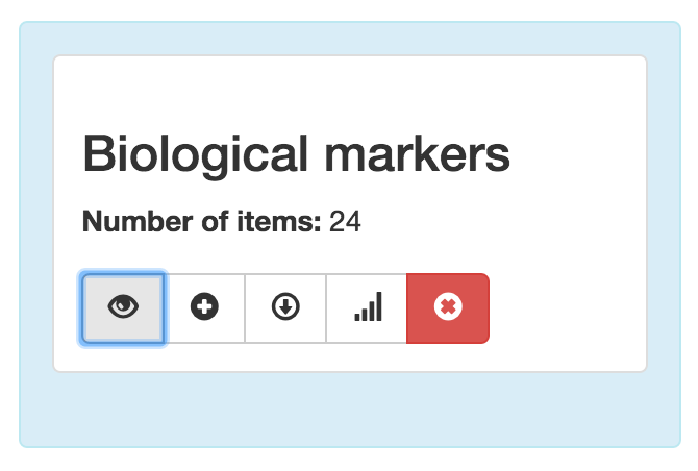
\includegraphics[width=5.5cm]{CreateCollectionsOut.eps}}
	\subfigure[]{\includegraphics[width=3cm]{inputFormStructuredDataOut.eps}}
	\subfigure[]{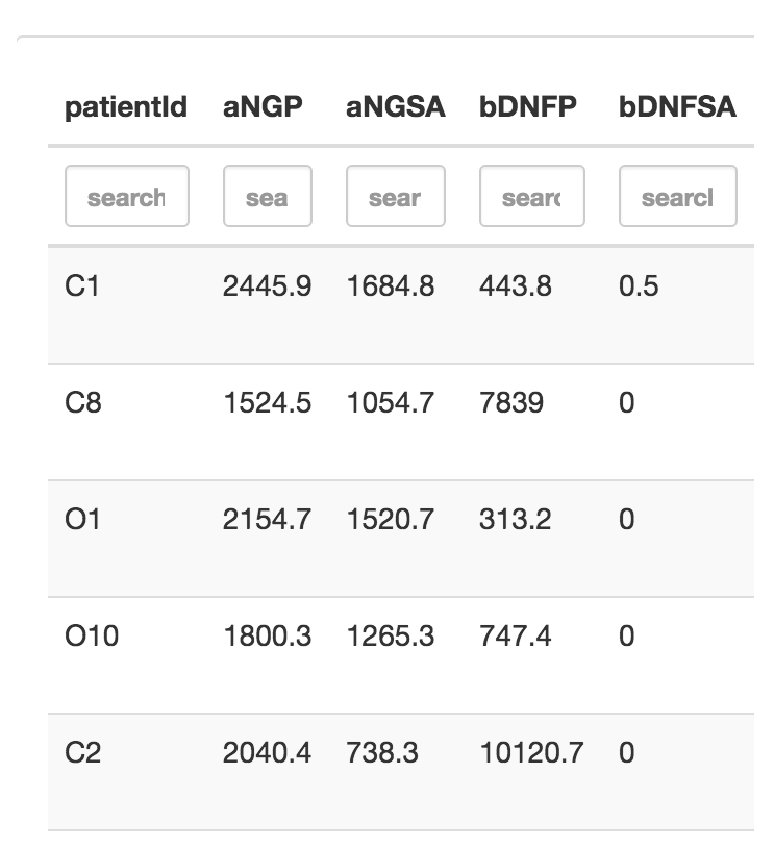
\includegraphics[width=3cm]{ImportDataFromSpreadSheetsOut.eps}}
	\caption[Import and generate clinical data]{a) Create a group or collection for clinical data. b) Forms or questionnaire. c) clinical data visualization.}
	\label{fig:gnerateClinicalData}
\end{figure} 

Figure \ref{fig:queryAndSelect}.a shows a view where the user can select different clinical variables, in this case, the variables correspond to genetic data
acquired for this study. Figure \ref{fig:queryAndSelect}.b shows patient selection. Figure \ref{fig:queryAndSelect}.c shows a plot using the selected 
variables in the clinical data and patient section. 

\begin{figure}
	\centering 
	\subfigure[]{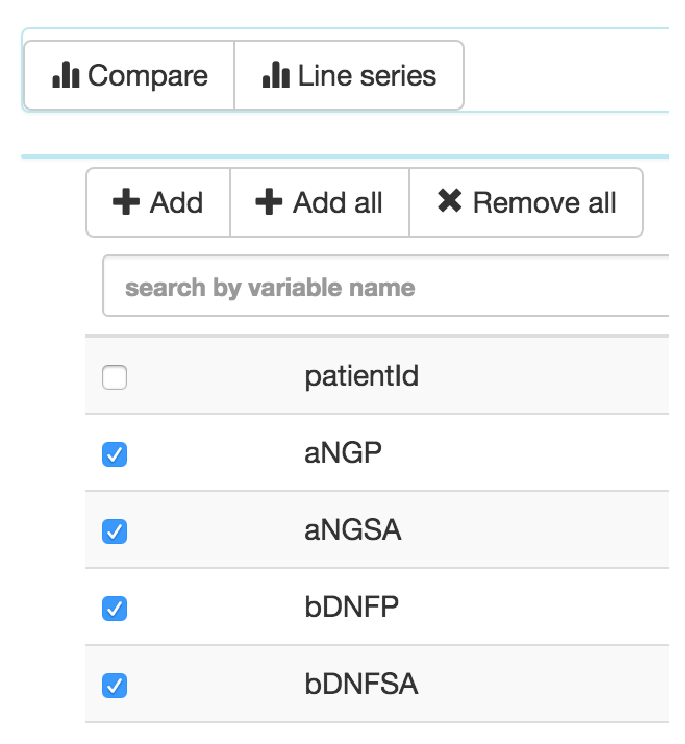
\includegraphics[width=3cm]{QueryAndFilterImportedDataOut.eps}}
	\subfigure[]{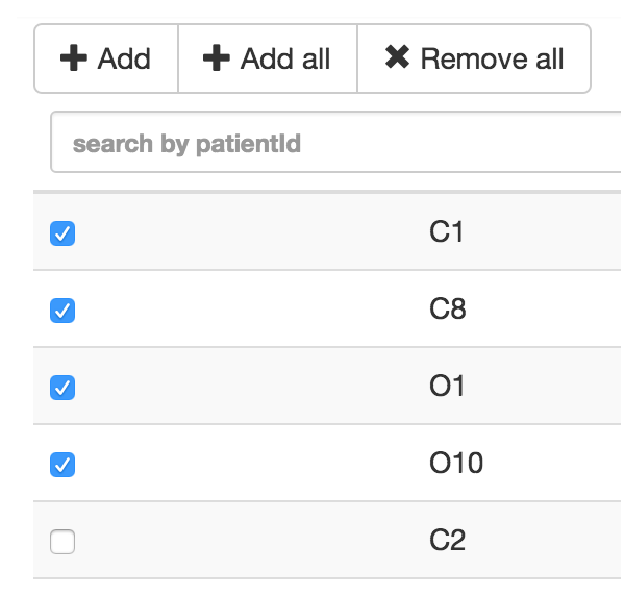
\includegraphics[width=3cm]{SelectPatientsOut.eps}}
	\subfigure[]{\includegraphics[width=7cm]{PlotOfControlPatientsForSomeProteinsOut.eps}}
	\caption[Import and generate clinical data]{a) Query and select clinical data. b) Query and select patients. c) Plot the selected data}
	\label{fig:queryAndSelect}
\end{figure} 

The plot produced in figure \ref{fig:queryAndSelect}.c is an interactive plot where the user can select a line and/or the legend on top 
in order to retrieve morphological data from the database. Figure \ref{fig:3DVisualizationOfCondyle} shows a drop down menu that is populated 
with the patient's data and the visualization of the structure in the interactive 3D viewer.

\begin{figure}
	\centering 
	\includegraphics[width=7cm]{3DVisualizationOfCondyleOut.eps}
	\caption[Visualization]{Condyle visualization in 3d}
	\label{fig:3DVisualizationOfCondyle}
\end{figure}

\section{CONCLUSIONS} 

The current state of the application allows gathering clinical data and morphological data in a structured manner. 
The tools and plugins described shown in Figure \ref{fig:serverArchitectureOut} have been published\footnote{\url{https://www.npmjs.com/~juanprietob}} and are available for installation with the Node package manager (npm). 
The current implementation of shiny-tooth has been deployed in the EC2 container and is available here\footnote{\url{https://ec2-52-42-49-63.us-west-2.compute.amazonaws.com:8180}}. The access to the data is restricted and will only be allowed after authorization from the project managers. 

%\acknowledgments

%%%%%%%%%%%%%%%%%%%%%%%%%%%%%%%%%%%%%%%%%%%%%%%%%%%%%%%%%%%%%
%%%%% References %%%%%

\scriptsize
\bibliography{report}   %>>>> bibliography data in report.bib
\bibliographystyle{spiebib}   %>>>> makes bibtex use spiebib.bst

\end{document} 
